\documentclass[a4paper]{article}

\usepackage[english]{babel}
\usepackage[utf8]{inputenc}
\usepackage{amsmath}
\usepackage{graphicx}
\usepackage{listings}
\usepackage{hyperref}
\hypersetup{
    colorlinks=true,
    linkcolor=blue,
    filecolor=magenta,      
    urlcolor=cyan,
}
\usepackage[colorinlistoftodos]{todonotes}

\title{\vspace{-5em}Multi Agent Systems Report 1 - Group 8}
\date{\today}

\author{Andrea Scorza, Diego Staphorst, Erik Lokhorst, Ingmar van der Geest}

\begin{document}
\maketitle

\begin{abstract}
This is the first report for the negotiation agent project for the course Multi-Agent Systems at Utrecht University. In the report, the Pareto efficient frontier is calculated and visualized. Also, two different negotiations with various agents are analyzed and visualized. 
\end{abstract}

\section{Computing the Pareto efficient frontier}
To visualize the Pareto efficient frontier, we manually calculated utility values for each preference in Excel. In Python, we were able to manipulate the data to get all the possible bids. With \href{https://sirinnes.wordpress.com/2013/04/25/pareto-frontier-graphic-via-python/}{Pareto frontier graphic via python} we were able to visualize the bids and Pareto Frontier, see figure \ref{fig:Pareto efficient figure} in the supplementary figures for the result.
\section{Analysis of negotiations between various agents}

\subsection{Single negotiation between two simple agents}
The negotiation between two single agents lasted 17 rounds and ended with an agreement where the utility gained by the agents was: $u(a_1) = 0.777$ and $u(a_2) = 0.510$. The strategy of both agents is to bid randomly until an agreement is reached, no optimization of utility takes place, see figure \ref{fig:Simple vs simple agents} for the visualized negotiation. There was no Pareto optimal outcome reached (distance to Pareto = 0.199), if this would happen in this scenario it would be purely coincidental.

\subsection{Single negotiation between Boulware agent and Conceder agent}
The negotiation lasted 83 rounds and ended with an agreement where $u(b) = 0.975$ and $u(c) = 0.495$. The strategy of the Boulware agent is to bid its maximum utility (u=1) up until the last rounds, where it slowly starts to concede. The strategy of the Conceder agent is to begin bidding its maximum utility (u=1) and in subsequent rounds lower its utility until an agreement is reached see figure \ref{fig:Boulware vs Conceder agent}, for the visualized negotiation. A Pareto optimal outcome is reached (distance to Pareto = 0.000). In different negotiations with different preference profiles, a Pareto optimal outcome was also reached. The Boulware agent performs very well against the Conceder agent because the Conceder will keep lowering its utility until it finds an agreement, at the same time the Boulware agent can simply stick with its near-optimal utility. 

\newpage
\section{\vspace{-1em}Supplementary figures}
\begin{figure}[h!]
\centering
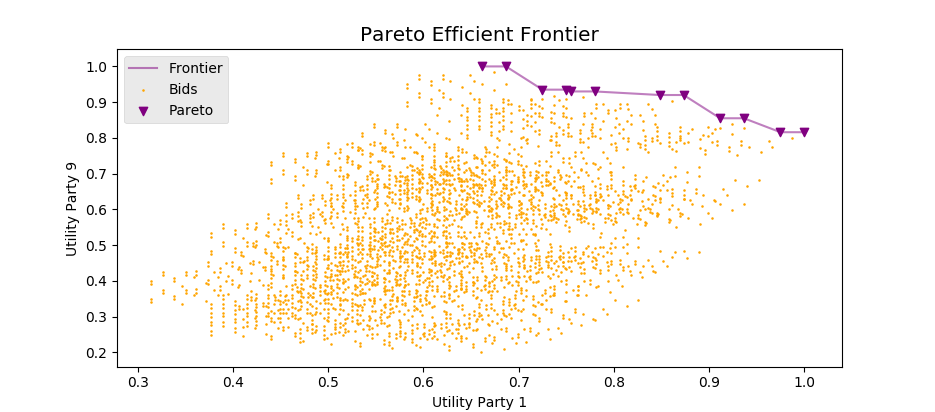
\includegraphics[width=125mm]{pareto_efficient.png}
\caption{Pareto efficient frontier including the bids generated with matplotlib in Python 3.7. The preferences of party 1 and party 9 were used.}
\label{fig:Pareto efficient figure}
\end{figure}

\begin{figure}[h!]
\centering
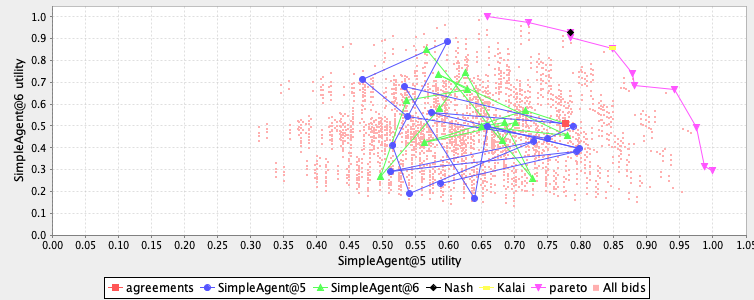
\includegraphics[width=125mm]{simplevssimple.png}
\caption{Results graph of the negotiation between two simple agents in Genius. The references of party 1 and party 2 were used.}
\label{fig:Simple vs simple agents}
\end{figure}

\begin{figure}[h!]
\centering
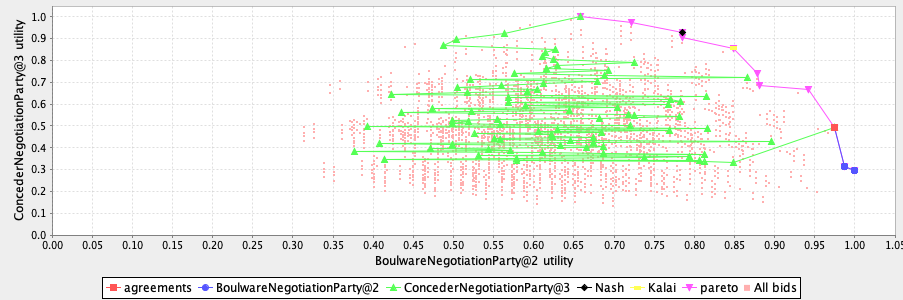
\includegraphics[width=125mm]{boulvsconcede.png}
\caption{Graph of the negotiation between the Boulware vs Conceder agents in Genius. The references of party 1 and party 2 were used.}
\label{fig:Boulware vs Conceder agent}
\end{figure}
\end{document}